\documentclass[a4paper,11pt]{article}
\usepackage[a4paper, left=1.5cm, right=1.5cm, top=2.0cm, bottom=3.5cm, headsep=1.2cm]{geometry}
\usepackage{polski}
\usepackage{amssymb}
\usepackage[utf8]{inputenc}
\prefixing
\usepackage{latexsym}
\usepackage{graphicx}
\usepackage{hyperref}
\author{Klaudia Balcer}
\title{Modele mieszane}
\frenchspacing
\begin{document}
\maketitle
\begin{center}
Zaawansowane Modele Liniowe

Raport 6
\end{center} 

\pagebreak

\section{Wizualizacja dopasowania modeli do danych}

%\textbf{Dopadowanie do danych modelu z losowym interceptem}

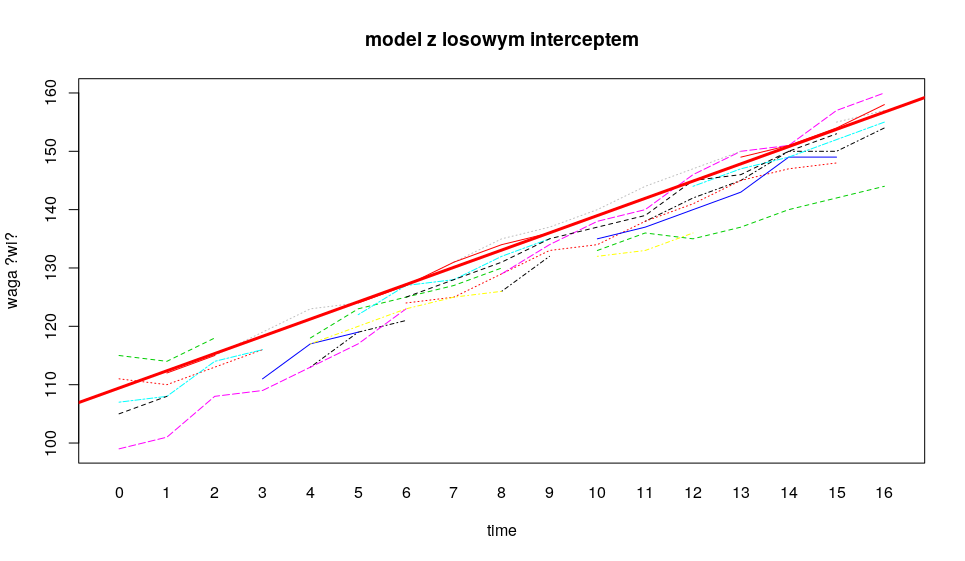
\includegraphics[scale=.67]{Int.png} 

%\textbf{Dopadowanie do danych modelu z losowym interceptem i slopem}

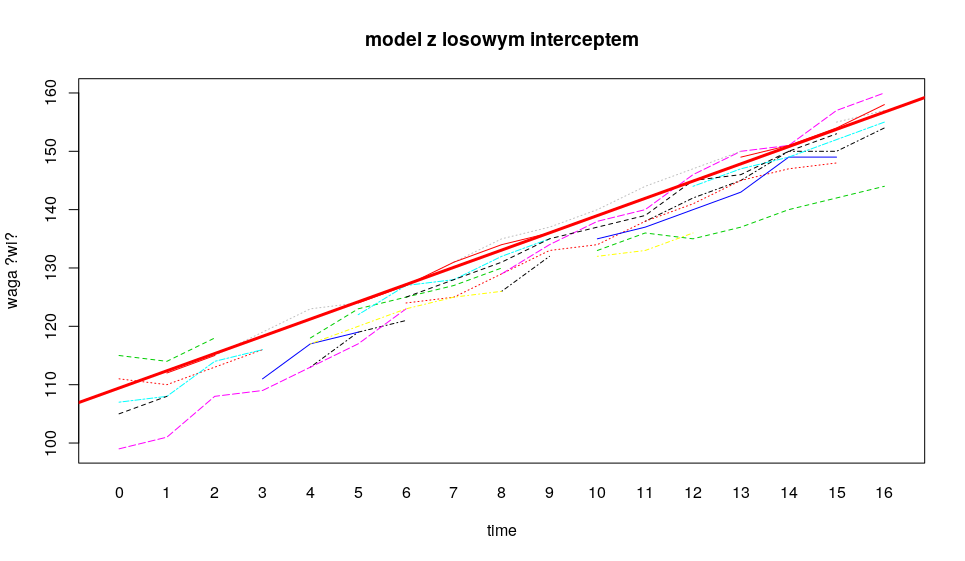
\includegraphics[scale=.67]{IntS.png} 

\pagebreak

\section{Równania dla populacji i osobników w poszczególnych modelach}

\begin{tabular}{|c|c|c|} \hline
  & model z losowym interceptem & model z losowym interceptem i slopem \\ \hline
równanie dla populacji & & \\ \hline
równanie dla osobnika & & \\ \hline

\end{tabular}
\end{document}